%File principale del documento su cui invocare la compilazione, vedi "istruzioni.txt" per più info

%Preambolo: la parte prima del \begin{document}
\documentclass[12pt,a4paper]{article} %formato del documento e grandezza caratteri

%Input del file metadata.tex della cartella locale "res/"
%lista di comandi presenti in template_latex.tex, da qui posso essere modificati secondo le esigenze

\newcommand{\DocTitle}{Verbale interno 2019-11-18} %variabile usata dal file template_latex.tex per settare il titolo del documento
%\newcommand{\DocAuthor}{Progetto "Predire in Grafana"} %variabile usata dal file template_latex.tex per settare l'autore del documento
\newcommand{\DocDate}{18 Novembre 2019} %variabile usata dal file template_latex.tex; Impostata manualmente, altrimenti ad ogni compilazione viene messa la data del giorno di compilazione.
\newcommand{\DocDesc}{Resoconto dell'incontro del gruppo \textit{VRAM Software} tenutosi in data 2019-11-18} %variabile usata dal file template_latex.tex per settare la descrizione del documento
\newcommand{\ver}{27.0.0} %variabile usata dal file template_latex.tex per settare la versione del documento
\newcommand{\app}{Toffoletto Massimo} %variabile usata dal file template_latex.tex per settare l'approvatore del documento
\newcommand{\red}{Dalla Libera Marco} %variabile usata dal file template_latex.tex per settare il redattore del documento
\newcommand{\test}{Schiavon Rebecca} %variabile usata dal file template_latex.tex per settare il verificatore del documento
\newcommand{\stat}{Approvato} %variabile usata dal file template_latex.tex per settare lo stato del documento
\newcommand{\use}{Interno} %variabile usata dal file template_latex.tex per indicare l'uso del documento %Contiene le varibili che descrivono il documento

%Input di file di configurazione presi dalla cartella "Template-LaTeX/config/", uguali per tutti i documenti
%Attenzione bisogna impostare il percorso del file!
% Tutti i pacchetti usati, da inserire nel preambolo prima delle configurazioni

\usepackage[T1]{fontenc} %Permette la sillabazione su qualsiasi testo contenente caratteri
\usepackage[utf8]{inputenc} %Serve per usare la codifica utf-8
\usepackage[english,italian]{babel} %Imposta italiano lingua principale, inglese secondaria. Es. serve per far apparire "indice" al posto di "contents"

\usepackage{graphicx} %Serve per includere le immagini

\usepackage[hypertexnames=false]{hyperref} %Gestisce i riferimenti/link. Es. Serve per rendere clickabili le sezioni dell'indice

\usepackage{float} %Serve per migliore la definizione di oggetti fluttuanti come figure e tabelle. Es. poter usare l'opzione [H] nelle figure ovvero tenere fissate le immagini che altrimenti LaTeX si sposta a piacere.

\usepackage{listings} %Serve per poter mettere snippets di codice nel testo

\usepackage{lastpage} %Serve per poter introdurre un'etichetta a cui si può fare riferimento Es. piè di pagina; poter fare " \rfoot{\thepage\ di \pageref{LastPage}} "

\usepackage{fancyhdr} %Per header e piè di pagina personalizzati

%Sono alcuni package che potranno esserci utili in futuro
%\usepackage{charter}
%\usepackage{eurosym}
\usepackage{subcaption}
%\usepackage{wrapfig}
%\usepackage{background}
\usepackage{longtable} % tabella che può continuare per più di una pagina
\usepackage[table]{xcolor} % ho dovuto aggiungere table in modo da poter colorare le row della tabella, dava: undefined control sequences
%\usepackage{colortbl}

\usepackage{dirtree} % usato per creare strutte tree-view in stile filesystem
\usepackage{xspace} % usato per inserire caratteri spazio
\usepackage[official]{eurosym}
\usepackage{pdflscape} %Inclusione pacchetti
% Configurazioni varie, da inserire nel preambolo dopo i pacchetti

\hypersetup{hidelinks} %serve per nascondere riquadri rossi che circondano i link 

\lstset{literate= {à}{{\`a}}1 } %Permette di usare lettere accentate nei listings

\pagestyle{fancy} %Imposto stile pagina
\fancyhf{} %Reset, se lo tolgo LaTex mette impostazioni di default (p.es numerazione pagine di default)


\lhead{
\includegraphics[scale=0.25]{img/logo_header.png}} %Left header che compare in ogni pagina
%\rhead{\leftmark} %Nome della top-level structure (p.es. Section in article o Chapter in book) in ogni pagina
\rhead{\DocTitle\ v. \ver} %Right header

\newcommand{\glo}{$_G$} %Comando per aggiungere il pedice G
\newcommand{\glosp}{$_G$ } %Comando per aggiungere il pedice G con spazio

\newcommand\Tstrut{\rule{0pt}{2.6ex}} % top padding
\newcommand\Bstrut{\rule[-0.9ex]{0pt}{0pt}} % bottom padding
\newcommand{\TBstrut}{\Tstrut\Bstrut} % top & bottom padding

%Setto il colore dei link
%\hypersetup{
%	colorlinks,
%	linkcolor=[HTML]{404040},
%	citecolor={purple!50!black},
%	urlcolor={blue!50!black}
%}

%Tabelle e tabulazione (può tornare utile)
%\setlength{\tablcolsep}{10pt}
%\renewcommand{\arraystretch}{1.4}

%Comando per aggiungere le pagine di ogni sezione
%\newcommand{\newSection}[1]{%
%	\input{res/sections/#1}
%}

% Comandi per aggiungere padding a parole contenute nella tabella; è una specie di strut (un carattere invisibile)
%\newcommand\Tstrut{\rule{0pt}{2.6ex}} % top padding
%\newcommand\Bstrut{\rule[-0.9ex]{0pt}{0pt}} % bottom padding
%\newcommand{\TBstrut}{\Tstrut\Bstrut} % top & bottom padding  %Configurazione pacchetti

\begin{document}
	%Input del file "frontmatter" preso dalla cartella "Template-LaTeX/config/", uguale per tutti i documenti
	%Attenzione bisogna impostare il percorso del file!
	% #### FRONTESPIZIO (frontmatter) ####
\setlength{\headheight}{33pt} %Distanzia l'header
\pagenumbering{gobble} %Toglie il numero di pagina
\begin{titlepage}
	\begin{center}
		
\includegraphics[scale=0.6]{img/logo.png} \\ %Logo
		\vspace{0.4cm} %Aggiunge uno spazio verticale di 0.5 cm
		
		{\LARGE Progetto "Predire in Grafana"} \\ %Nome progetto
		\vspace{0.4cm} %Attenzione a mettere il punto e NON la virgola
		
		{\Huge \textbf{\DocTitle}} \\ %Titolo, prende variabile definita in metadata.tex
		\vspace{0.4cm}
		
		\DocDate \\ %Data, prende variabile definita in metadata.tex
		\vspace{0.4cm}
		
		%Allineamento colonne: l=left r=right c=center, 
		%va specificato per ogni colonna
		%Se si vuole la riga tra colonne mettere "|"
		
		\begin{tabular}{r | l} %Elementi colonne separate da "&", le righe finiscono con "\\"
			Versione             & \ver \\
			Approvazione         & \app \\ 
			Redazione            & \red \\
			Verifica             & \test \\
			Stato                & \stat \\
			Uso                  & \use \\
		    Destinato a          & Zucchetti \\
						         & Prof. Vardanega Tullio\\
						         & Prof. Cardin Riccardo\\
			Email di riferimento & vram.software@gmail.com
		\end{tabular}
		\vfill
		\textbf{Descrizione} \\
		\DocDesc
	\end{center}
\end{titlepage}
\clearpage

% #### Impostazione header, footer  e numerazione pagine ####
\pagenumbering{arabic} %Pagine con i numeri arabi + reset a 1
\renewcommand{\footrulewidth}{0.4pt} %Di default footrulewidth==0 e quindi è invisibile, di default \headrulewith==0.4pt
\rfoot{\thepage\ di \pageref{LastPage}} %Pagina n di m, con numeri Arabi; usa il pacchetto "lastpage", in caso non sia possibile usare tale pacchetto mettere al fondo dell'ultima pagina "\label{LastPage}"

% #### Tabella dei log ####
% \textbf = grassetto; \Large = font più grande
% \rowcolors{quanti colori alternare}{colore numero riga pari}{colore numero riga dispari}: colori alternati per riga
% \rowcolor{color}: cambia colore di una riga
% p{larghezza colonna}: p è un tipo di colonna di testo verticalmente allineata sopra, ci sarebbe anche m che è centrata a metà ma non è precisa per questo utilizzo TBStrut; la sintassi >{\centering} indica che il contenuto della colonna dovrà essere centrato
% \TBstrut fa parte di alcuni comandi che ho inserito in config.tex che permetto di aggiungere un po' di padding al testo
% \\ [2mm] : questra scrittura indica che lo spazio dopo una break line deve essere di 2mm
% 

%\setcounter{secnumdepth}{0}
%\hfill \break
%\textbf{\Large{Diario delle modifiche}} \\


\addtocontents{toc}{\protect\setcounter{tocdepth}{0}} %Inserire questo per escludere una sezione dall'indice.

\section*{Registro delle modifiche} %Asterisco per fare sezione non numerata
\rowcolors{2}{gray!25}{gray!15}
\begin{longtable} {
		>{\centering}p{17mm} 
		>{\centering}p{19.5mm}
		>{\centering}p{24mm} 
		>{\centering}p{24mm} 
		>{}p{32mm}}
	\rowcolor{gray!50}
	\textbf{Versione} & \textbf{Data} & \textbf{Nominativo} & \textbf{Ruolo} & \textbf{Descrizione} \TBstrut \\
	14.7.0 & 2020-04-09 & Stantagiuliana Vittorio, Toffoletto Massimo e Spreafico Alessandro & \textit{Progettista}, \textit{Verificatore} e \textit{Responsabile di progetto} & Stesura, verifica e approvazione documento. \TBstrut \\ [2mm]
\end{longtable}

\addtocontents{toc}{\protect\setcounter{tocdepth}{4}} %Inserire questo per ripristinare il normale inserimento delle sezioni nell'indice. 4 significa fino al paragrah
\clearpage

% #### INDICE (tableofcontents) ####
\tableofcontents %Provoca la stampa dell'indice
\clearpage

\setcounter{secnumdepth}{4} %Permette di andare fino alla profondità del paragraph con la numerazione delle sezioni %Imposta il frontespizio, l'indice, header e footer
	
	\listoftables
	\clearpage
	\listoffigures
	\clearpage
	
	%Tutte le sezioni del documento
	%\input{res/inserire nome sezione 1} 
	% ...

	\section{Introduzione}
    \subsection{Scopo del documento}
        L'obiettivo di questo documento è riportare in modo puramente tecnico le scelte architetturali, strutturali e logiche intraprese dal gruppo \textit{VRAM Software} nel corso dello sviluppo del progetto \textit{Predire in Grafana}. Tale allegato sarà quindi corredato di vari diagrammi UML 2.x (classe, package e sequenza) che dimostreranno i vari design pattern adottati, la struttura del prodotto e i suoi scenari di esecuzione.
    \subsection{Scopo del prodotto}
        Il prodotto che il gruppo \textit{VRAM Software} sta approfondendo prevede lo sviluppo di un applicativo esterno e di un plug-in per la piattaforma di analisi Grafana\glosp per la predizione di dati tramite gli algoritmi di support vector machine (SVM) e di regressione lineare (RL). L'applicativo esterno fungerà da trainer generando un file JSON (predittore) partendo da dei dati in CSV a cui viene applicato l'algoritmo di predizione scelto dall'utente. Il file JSON ottenuto sarà poi inserito nel software Grafana tramite l'apposito plug-in e, dopo aver associato i nodi che si vogliono analizzare con i rispettivi predittori, sarà possibile visualizzare la previsione sul grafico della dashboard di Grafana. È inoltre presente la possibilità di salvare suddetti dati su un database InfluxDB. In tal modo il gruppo \textit{VRAM Software} insieme al proponente \textit{Zucchetti} punta ad agevolare l'attività di DevOps fornendo un valido strumento di predizione e monitoraggio dei dati.
    \subsection{Riferimenti}
        \subsubsection{Normativi}
            \begin{itemize}
                \item \textbf{Norme di Progetto}: \textit{Norme di Progetto v. 27.0.0};
                \item \textbf{Capitolato}\glosp \textbf{d'appalto}: \textit{C4 - Zucchetti - Predire in Grafana} \\
                 \url{https://www.math.unipd.it/~tullio/IS-1/2019/Progetto/C4.pdf}.
            \end{itemize}
        \subsection{Informativi}
        \begin{itemize}
        	\item \textbf{Analisi dei Requisiti}: \textit{Analisi dei Requisiti v. 27.0.0}
        \end{itemize}
        \subsection{Tecnici}
            \begin{itemize}
                \item \textbf{TypeScript}: \url{https://www.typescriptlang.org/docs/home.html};
                \item \textbf{JavaScript}: \url{https://developer.mozilla.org/it/docs/Web/JavaScript};
                \item \textbf{AngularJS}: \url{https://docs.angularjs.org/api};
                \item \textbf{React}: \url{https://it.reactjs.org/docs}.
            \end{itemize}
	\section{Requisiti di sistema}
Vengono riportati i requisiti minimi per lo sviluppo e l'esecuzione del nostro prodotto. Essi sono uguali sia per l'applicazione esterna che per il plug-in.

\subsection{Requisiti hardware}
I requisiti hardware minimi che devono essere soddisfatti per garantire un corretto funzionamento sono:
\begin{itemize}
	\item RAM: 2 GB;
	\item Memoria interna libera: 5 GB;
	\item Processore: minimo dual core.
\end{itemize}

\subsection{Sistemi operativi}
Il prodotto è stato sviluppato, testato e utilizzato sui seguenti sistemi operativi, perciò è garantita la compatibilità:
\begin{itemize}
	\item Distribuzioni Gnu/Linux post 2019 basate su DEB o RPM;
	\item macOS v. 10.15;
	\item Windows v. 10.
\end{itemize}

\subsection{Browser compatibili}
Il plug-in è stato sviluppato, testato e utilizzato sui seguenti browser perciò ne è garantita la compatibilità:
\begin{itemize}
	\item Google Chrome v. 58;
	\item Mozilla Firefox v. 54;
	\item Microsoft Edge v. 14;
	\item Microsoft Internet Explorer v. 11;
	\item Safari v. 10;
	\item Opera v. 55.
\end{itemize}
Per l'applicazione esterna alla piattaforma Grafana viene utilizzato Chromium che è integrato, dunque non è necessario l'utilizzo di un browser.
Per ottenere un corretto funzionamento del prodotto è richiesta l'abilitazione di Javascript.

  	\section{Architettura}
	Il nostro prodotto è composto da un plug-in sviluppato per la piattaforma Grafana e un'applicazione esterna a quest'ultima. L'analisi dell'architettura sarà quindi divisa per questi due componenti.
	\subsection{Plug-in interno a Grafana}
		Per poter apprezzare la suddivisione del prodotto viene riportato il diagramma dei Package, allegato nel file DOBBIAMO_DEVIDERE_IL_NOME.PNG, che rappresenta le dipendenze definite ad alto livello tra le componenti.
		\subsubsection{Progettazione architetturale}
		Per la progettazione architetturale del plug-in si è deciso di utilizzare il design pattern MVC. Abbiamo preso questa decisione perché si adatta bene allo sviluppo di software all'interno della piattaforma Grafana. In particolare è così strutturata:
		\begin{itemize}
			\item \textbf{Model}: all'interno del Model gestiamo la business logic del nostro prodotto, più in dettaglio la predizione dei dati sulla base degli algoritmi che abbiamo implementato, la lettura dei dati da utilizzare e la scrittura dell'esito della loro elaborazione tramite un database Influx, considerato lo standard per la piattaforma Grafana;
			\item \textbf{View}: all'interno della View gestiamo la presentation logic del nostro prodotto, più in dettaglio la creazione di un pannello della dashboard di Grafana e le sue interazioni con l'utente;
			\item \textbf{Controller}: all'interno del Controller gestiamo l'application logic del nostro prodotto, più in dettaglio la necessaria trasformazione dei dati forniti dall'utente in un formato utilizzabile dai componenti del Model.
		\end{itemize}
		In allegato forniamo il diagramma delle classi nel file DOBBIAMO_DECIDERE_IL_NOME.PNG .
		\subsubsection{Progettazione di dettaglio}
			\paragraph{Model}
			Come prima cosa all'interno del modello abbiamo inserito gli algoritmi di predizione. Per la progettazione dei componenti che li implementano, abbiamo deciso di privilegiare l'estensibilità creando un'interfaccia \textit{AlgorithmPrediction} che da contratto fornisce il metodo \textit{predict(dataset, configuration, influxParams)} che riceve in input i dati e la configurazione per eseguire l'algoritmo e i parametri per connettersi e salvare il risultato su InfluxDB.
			In questo modo è possibile implementare nuovi algoritmi a partire dalla suddetta interfaccia, rispettando i parametri espressi. Noi abbiamo implementato gli algoritmi Support Vector Machine e Regressione lineare e quindi abbiamo fornito due implementazioni concrete dell'interfaccia.
			\textit{SvmPrediction} è la classe che implementa l'algoritmo SVM ed importa la libreria ml-modules mentre \textit{RlPrediction} è quella che implementa RL ed importa LinearRegression dalla libreria \textit{regression.module}. Entrambe sono caratterizzate da un campo dati writeInflux che rappresenta un oggetto di Classe WriteInflux che viene quindi istanziato nel costruttore. Questo rappresenta una dipendenza di tipo composizione e risulta essere esplicita. [INSERIRE DIAGRAMMA]
			Infine la classe concreta \textit{WriteInflux} che importa la libreria \textit{node-influx} rappresenta la connessione con il database influxDB e di conseguenza una dipendenza con esso. In questo caso non si è scelto di fornire un'interfaccia in quanto all'intero di Grafana viene utilizzato questo db come standard. Presenta due metodi per la scrittura sul database rispettivamente \textit{WriteArrayToInflux(data, timeStamp)} che permette di scrivere i dati e \textit{writeStampsToInflux(point, timeStamp)} che permette di inserire il timeStamp, caratteristico di un database TimeScale come Influx. 
			[INSERIRE DIAGRAMMA]
			Per la comunicazione dei dati tra Model e View ci appoggiamo al funzionamento di Grafana che la implementata utilizzando un design pattern Observer. 
			\paragraph{View}
			All'interno della vista abbiamo inserito la componente Panel rappresentata dalla classe \textit{PanelCtrl} che estende la classe \textit{MetricsPanelCtrl} di Angular. Essa permette la visualizzazione dei risultati delle query su Influx.
			Inoltre è presente la classe \textit{SelectInfluxDBCtrl} che rappresenta la componente di ricezione della datasource definita e connessa dall'utente tramite l'interfaccia grafica. Essa è in relazione di composizione con \textit{PanelCtrl} che la contiene e ne gestisce il ciclo di vita; infatti non ha senso di esistere al di fuori del pannello che permette la visualizzazione dei dati che legge.
			Per implementare i grafici, invece, abbiamo deciso di utilizzare un componente della libreria Plotly che importiamo e gestiamo interamente dentro \textit{PanelCtrl}.
			Infine nella classe \textit{PanelCtrl} è presente un campo dati che rappresenta un oggetto di tipo ProcessData che viene gestito interamente. Perciò è presente una dipendenza di composizione tra queste due classi che definisce anche la relazione che sussiste tra View e Model del nostro prodotto. [INSERIRE DIAGRAMMA]
			\paragraph{Controller}
			All'interno del controller viene implementata la mappatura tra i dati e le richieste ricevute dalla View e le chiamate alla business logic per la loro esecuzione. Abbiamo deciso di implementare un design pattern strategy ottenendo la seguente struttura:
			\begin{itemize}
				\item \textbf{ProcessData}: questa è una classe concreta che rappresenta il context e al suo interno viene scelto, sulla base dei dati e della richieste ricevute, quale strategia seguire, che in questo caso è rappresentata da quale algoritmo di predizione processare;
				\item \textbf{PerformPrediction}: questa è un'interfaccia che rappresenta la strategia astratta. Essa definisce il contratto che un componente che processa i dati per un determinato algoritmo deve avere per essere tale;
				\item \textbf{ProcessSvm}: questa è una classe concreta che implementa \textit{PerformPrediction} e rappresenta il componente che esegue la mappatura e il controllo dei dati per fornirli all'algoritmo di predizione Svm;
				\item \textbf{ProcessRl}: questa è una classe concreta che implementa \textit{PerformPrediction} e rappresenta il componente che esegue la mappatura e il controllo dei dati per fornirli all'algoritmo di predizione Rl.
			\end{itemize}
			All'interno di \textit{ProcessSvm} e \textit{ProcessRl} è presente un attributo rispettivamente SvmPredicter e RlPredicter che definisce una dipendenza di tipo composizione e di conseguenza il collegamento tra Controller e Model. [INSERIRE DIAGRAMMA]
	\subsection{Applicazione esterna alla piattaforma Grafana}
	Per poter apprezzare la suddivisione del prodotto viene riportato il diagramma dei Package, allegato nel file DOBBIAMO_DEVIDERE_IL_NOME.PNG, che rappresenta le dipendenze definite ad alto livello tra le componenti.
		\subsubsection{Progettazione architetturale}
			Per la progettazione architetturale dell'applicazione esterna a Grafana si è deciso di utilizzare il design pattern MVVM. Abbiamo preso questa decisione perché si adatta molto bene alle tecnologie che utilizziamo ovvero React ed Electron. In particolare è così strutturata:
		\begin{itemize}
			\item \textbf{Model}: all'interno del Model gestiamo la business logic dell'applicazione, più in dettaglio eseguiamo l'addestramento dei dati attraverso gli algoritmi di predizione e le operazioni di input-output attraverso i file;
			\item \textbf{View}: all'interno della View gestiamo la presentazione dei dati attraverso React;
			\item \textbf{ViewModel}: all'interno del ViewModel implementiamo il binding tra la vista ed il modello. Più in dettaglio il binding tra View e ViewModel ci viene fornito da Electron mentre quello tra Model e ViewModel viene implementato tramite l'utilizzo delle callback.
		\end{itemize}
		In allegato forniamo il diagramma delle classi nel file DOBBIAMO_DECIDERE_IL_NOME.PNG .
		\subsubsection{Progettazione di dettaglio}
			\paragraph{Model}
			Progettando il modello dell'applicazione esterna abbiamo riscontrato la necessità di utilizzare in due diversi casi un Template Method: \\
			\textbf{Read} \mbox{} \\ 
			Abbiamo notato che nella gestione dell'input, indipendentemente dall'estensione del file ricevuto, l'algoritmo per eseguire la lettura di quest'ultimo aveva uno scheletro comune. È stato quindi deciso di implementare un template method. La classe astratta Read implementa il metodo readFile(path, callback) che definisce l'algoritmo comune, esegue una lettura dal file system del file e chiama una funzione parser(data, callback) che viene implementata nelle classi concrete ReadCsv e ReadJson a seconda delle specifiche esigenze dell'estensione del file. La funzione readFile(path, callback) restituisce infine una stringa, mediante la chiamata della callback, contenente le informazioni lette. 
			[INSERIRE DIAGRAMMA]
			\textbf{Write} \mbox{} \\ 
			Progettando la gestione degli output ci si è accorti che indipendentemente dall'estensione del file da scrivere, l'algoritmo di scrittura aveva uno scheletro comune. È stato quindi deciso di implementare un template method per eventuali sviluppi futuri. La classe astratta Write implementa il metodo writeToDisk(path, name, data, notes, callback) che definisce l'algoritmo comune. Viene chiamata la funzione buildTrainedFile(result, notes), implementata nella classe concreta WriteJson, che restituisce una map<String, double> che rappresenta l'oggetto da scrivere nel file da dare in output. Viene poi chiamata la funzione parser(data, callback), implementata nella classe concreta WriteJson, che trasformerà questo oggetto in una stringa. Il metodo writeToDisk(path, name, data, notes, callback) riceverà infine questa stringa tramite la callback e la scriverà in un file da dare in output.
			[INSERIRE DIAGRAMMA]
			Inoltre abbiamo implementato gli algoritmi di predizione attraverso un'interfaccia \textit{AlgorithmTrainer}. Essa permette l'estensibilità a qualunque algoritmo purché rispetti il contratto definito. Attualmente abbiamo implementato \textit{SvmTrainer} e \textit{RlTrainer} ovvero le classi rispettivamente dell'addestramento di Svm ed Rl.
			Per le funzionalità sopra elencate, implementiamo l'invio delle notifiche alla ViewModel per l'aggiornamento dei dati tramite il meccanismo di callback.			
			\paragraph{View}
			La parte di presentazione dei dati verso l'utente è realizzata tramite dei componenti di React, contenuti nella classe principale App che li renderizza. Inoltre per la visualizzazione del grafico risultante dalla predizione abbiamo deciso di utilizzare la libreria D3. 
			La gestione dello stato dell'applicazione è delegata al ViewModel che si occupa di aggiornare lo stato che verrà poi renderizzato dalla vista. 	
			\paragraph{ViewModel}
			Nella parte di ViewModel dell'applicazione sono contenuti i dati da visualizzare nella vista e le operazioni che devono essere effettuate dal modello per soddisfare le richieste dell'utente. In particolare il ViewModel è legato alla vista tramite Electron che ne gestisce lo scambio di dati appoggiandosi al nostro componente EventManager e con il modello tramite il meccanismo di callback.
			Per il process dei dati abbiamo riscontrato la necessità implementare in tre diversi casi il design pattern strategy: \\
			\textbf{Reading} \mbox{} \\ 
			\begin{itemize}
				\item \textbf{ProcessReading}: questa è una classe concreta che rappresenta il context e al suo interno viene scelto, sulla base dei dati e della richieste ricevute, quale strategia seguire, che in questo caso è leggere un file Csv o un file Json;
				\item \textbf{PerformReading}: questa è un'interfaccia che rappresenta la strategia astratta. Essa definisce il contratto che un componente che legge un file in input deve avere per essere tale;
				\item \textbf{ProcessReadingCsv}: questa è una classe concreta che implementa \textit{PerformReading} e rappresenta il componente che esegue la lettura dei dati da un file Csv;
				\item \textbf{ProcessReadingJson}: questa è una classe concreta che implementa \textit{PerformReading} e rappresenta il componente che esegue la lettura dei dati da un file Json.
			\end{itemize}
			[INSERIRE DIAGRAMMA]
			\textbf{Writing} \mbox{} \\ 
			\begin{itemize}
				\item \textbf{ProcessWriting}: questa è una classe concreta che rappresenta il context e al suo interno viene scelto, sulla base dei dati e della richieste ricevute, quale strategia seguire, che in questo caso scrivere un file in base alla sua estensione;
				\item \textbf{PerformWriting}: questa è un'interfaccia che rappresenta la strategia astratta. Essa definisce il contratto che un componente che deve scrivere un file da dare in output deve avere per essere tale;
				\item \textbf{ProcessWritingJson}: questa è una classe concreta che implementa \textit{PerformWriting} e rappresenta il componente che esegue la scrittura dei dati su un file Json;
			\end{itemize}
			[INSERIRE DIAGRAMMA]
			\textbf{Training} \mbox{} \\ 
			\begin{itemize}
				\item \textbf{ProcessTraining}: questa è una classe concreta che rappresenta il context e al suo interno viene scelto, sulla base dei dati e della richieste ricevute, quale strategia seguire, che in questo caso è rappresentata da quale algoritmo di predizione addestrare;
				\item \textbf{PerformTraining}: questa è un'interfaccia che rappresenta la strategia astratta. Essa definisce il contratto che un componente che processa i dati per un determinato algoritmo deve avere per essere tale;
				\item \textbf{ProcessTrainingRl}: questa è una classe concreta che implementa \textit{PerformTraining} e rappresenta il componente che esegue la mappatura e il controllo dei dati per fornirli all'algoritmo di predizione Rl per eseguire il suo addestramento;
				\item \textbf{ProcessTrainingSvm}: questa è una classe concreta che implementa \textit{PerformTraining} e rappresenta il componente che esegue la mappatura e il controllo dei dati per fornirli all'algoritmo di predizione Svm per eseguire il suo addestramento.
			\end{itemize}
			[INSERIRE DIAGRAMMA]
	\section{Interazioni fra componenti}
	\subsection{Predizione e scrittura del risultato}
	Per rappresentare come interagiscono i componenti del nostro sistema per predire i dati e scrivere il risultato viene di seguito riportato un diagramma di sequenza che mostra l'esempio in cui l'algoritmo di predizione utilizzato è Support Vector Machine. Questo esempio risulta indicativo anche per l'algoritmo di predizione Regressione Lineare.  
	\mbox{}
	\begin{figure} [H]
		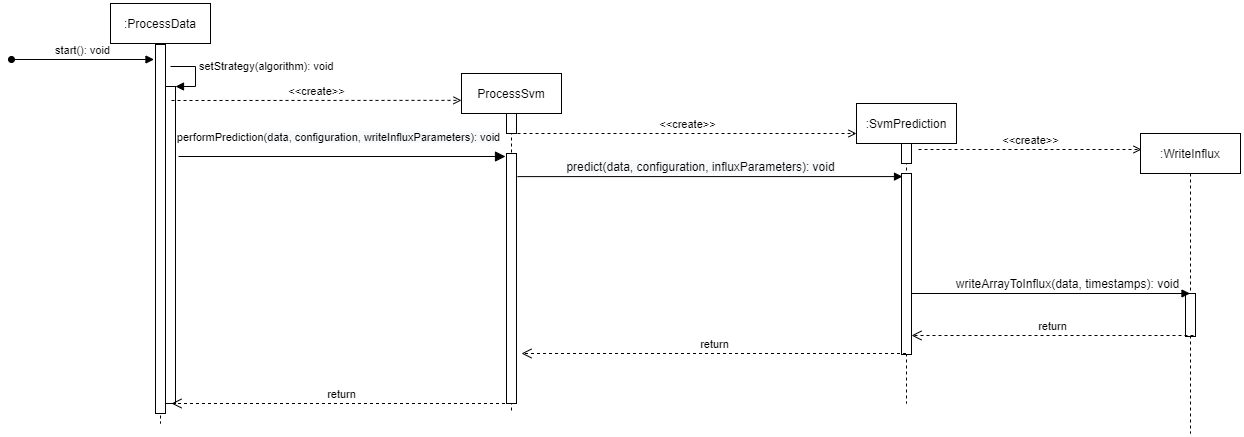
\includegraphics[width=\linewidth]{./img/Diagrammi/ds1.png}
		\caption{Diagramma di sequenza di predizione e scrittura del risultato}
	\end{figure}
	Un'istanza di ProcessData, ricevuto il messaggio onDataRecieved(), setta il suo attributo di strategia e, di conseguenza, crea un'istanza di ProcessSvm che crea un oggetto SvmPrediction che a sua volta crea un oggetto di WriteInflux.
	L'istanza di ProcessSvm esegue quindi il metodo performPrediction(data, configuration, writeInfluxParameters) che chiama il metodo predict(data, configuration,influxParametres) sull'oggetto di tipo SvmPrediction. Quest'ultimo, ricevuti i parametri in input, esegue la predizione e chiama il metodo writeArraytoInflux(data, timestamps) su un'istanza di WriteInflux che andrà a scrivere il risultato della previsione su un database Influx.
	
	\subsection{Addestramento dell'algoritmo}
	Per rappresentare come interagiscono i componenti del nostro sistema per addestrare l'algoritmo di previsione viene di seguito riportato un diagramma di sequenza che mostra l'esempio in cui l'algoritmo utilizzato è Support Vector Machine. Questo esempio risulta indicativo anche per l'algoritmo di predizione Regressione Lineare.  
	\mbox{}
	\begin{figure} [H]
		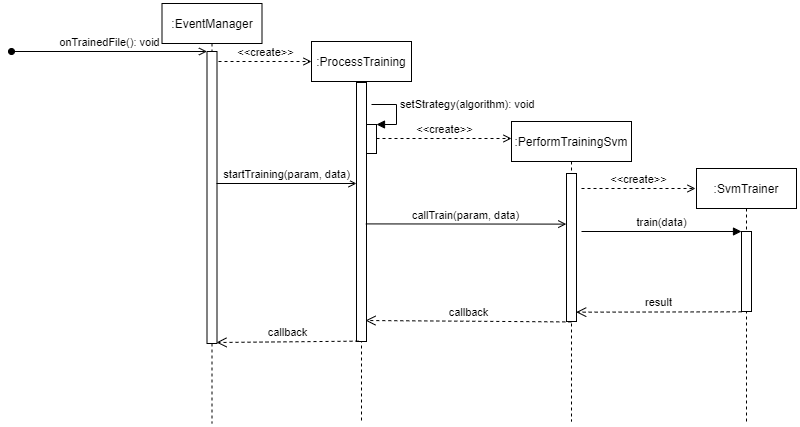
\includegraphics[width=\linewidth]{./img/Diagrammi/ds2.png}
		\caption{Diagramma di sequenza dell'addestramento dell'algoritmo}
	\end{figure}
	Un'istanza di EventManager, ricevuto il messaggio onTrainedFile(), crea un'istanza di ProcessTraining che setta il suo attributo di strategia e, di conseguenza, crea un'istanza di PerformTrainingSvm. Quest'ultima crea quindi un oggetto SvmTrainer.
	L'istanza EventManager esegue quindi una chiamata asincrona startTraining(param, data) sull'oggetto ProcessTraining. Esso a sua volta esegue la chiamata asincrona callTrain(param, data) sull'oggetto PerformTrainingSvm che chiama il metodo train(data) sull'oggetto SvmTrainer. Infine quest'ultimo ritornerà quindi il risultato dell'addestramento.
  	\section{Tracciamento}
    \subsection{Tracciamento requisiti funzionali}
        \rowcolors{2}{gray!25}{gray!15}
        \begin{longtable} {
            >{\centering}p{64.5mm} 
            >{}p{64.5mm}
            }
        \rowcolor{gray!50}
            \textbf{Requisito} & \textbf{Implementazione} \TBstrut \\
            R3F1 & Non implementato \TBstrut \\ [2mm]
            R3F1.1 & Non implementato \TBstrut \\ [2mm]
            R3F1.1.1 & Non implementato \TBstrut \\ [2mm]
            R3F1.1.2 & Non implementato \TBstrut \\ [2mm]
            R3F1.5 & Non implementato \TBstrut \\ [2mm]
            R3F1.6 & Non implementato \TBstrut \\ [2mm]
            R3F1.6.1 & Non implementato \TBstrut \\ [2mm]
            R3F1.6.2 & Non implementato \TBstrut \\ [2mm]
            R3F1.7 & Non implementato \TBstrut \\ [2mm]
            R3F1.2 & Non implementato \TBstrut \\ [2mm]
            R3F1.9 & Non implementato \TBstrut \\ [2mm]
            R3F1.10 & Non implementato \TBstrut \\ [2mm]
            R3F1.11 & Non implementato \TBstrut \\ [2mm]
            R3F1.12 & Non implementato \TBstrut \\ [2mm]
            R3F1.13 & Non implementato \TBstrut \\ [2mm]
            R3F1.14 & Non implementato \TBstrut \\ [2mm]
            R3F1.3 & Non implementato \TBstrut \\ [2mm]
            R3F1.4 & Non implementato \TBstrut \\ [2mm]
            R3F1.8 & Non implementato \TBstrut \\ [2mm]		
            R3F2 & Non implementato \TBstrut \\ [2mm]
            R3F2.1 & Non implementato \TBstrut \\ [2mm]
            R3F2.2 & Non implementato \TBstrut \\ [2mm]
            R3F2.3 & Non implementato \TBstrut \\ [2mm]
            R3F3 & Non implementato \TBstrut \\ [2mm]
            R3F17 & Non implementato \TBstrut \\ [2mm]	
            R1F4 & Implementato \TBstrut \\ [2mm]		
            R1F4.1 & Implementato \TBstrut \\ [2mm]		
            R1F4.1.1 & Implementato \TBstrut \\ [2mm]
            R1F4.1.2 & Implementato \TBstrut \\ [2mm]
            R1F4.8 & Implementato \TBstrut \\ [2mm]
            R1F4.9 & Implementato \TBstrut \\ [2mm]
            R1F4.9.1 & Implementato \TBstrut \\ [2mm]
            R1F4.9.2 & Implementato \TBstrut \\ [2mm]
            R1F4.10 & Implementato \TBstrut \\ [2mm]	
            R1F4.2 & Implementato \TBstrut \\ [2mm]
            R1F4.11 & Implementato \TBstrut \\ [2mm]
            R1F4.12 & Implementato \TBstrut \\ [2mm]
            R3F4.13 & Non implementato \TBstrut \\ [2mm]
            R3F4.14 & Non implementato \TBstrut \\ [2mm]
            R3F4.15 & Non implementato \TBstrut \\ [2mm]
            R3F4.16 & Non implementato \TBstrut \\ [2mm]		
            R1F4.4 & Implementato \TBstrut \\ [2mm]
            R1F4.5 & Implementato \TBstrut \\ [2mm]		
            R2F4.6 & Implementato \TBstrut \\ [2mm]		
            R1F4.7 & Implementato \TBstrut \\ [2mm]
            R1F5 & Non implementato \TBstrut \\ [2mm]
            R1F5.1 & Non implementato \TBstrut \\ [2mm]
            R1F5.2 & Non implementato \TBstrut \\ [2mm]
            R1F5.3 & Non implementato \TBstrut \\ [2mm]
            R2F6 & Non implementato \TBstrut \\ [2mm]
            R2F18 & Non implementato \TBstrut \\ [2mm]
            R1F19 & Implementato \TBstrut \\ [2mm]
            R1F7 & Implementato \TBstrut \\ [2mm]
            R1F21 & Implementato \TBstrut \\ [2mm]
            R1F8 & Implementato \TBstrut \\ [2mm]
            R1F9 & Implementato \TBstrut \\ [2mm]
            R1F9.1 & Implementato \TBstrut \\ [2mm]
            R1F9.2 & Implementato \TBstrut \\ [2mm]
            R3F9.3 & Non implementato \TBstrut \\ [2mm]
            R1F9.4 & Implementato \TBstrut \\ [2mm]
            R2F9.5 & Implementato \TBstrut \\ [2mm]
            R2F10 & Non implementato \TBstrut \\ [2mm]
            R1F11 & Implementato \TBstrut \\ [2mm]
            R1F12 & Implementato \TBstrut \\ [2mm]	
            R1F20 & Implementato \TBstrut \\ [2mm]	
            R2F13 &	Non implementato \TBstrut \\ [2mm]					
            R2F13.2 & Non implementato \TBstrut \\ [2mm]		
            R2F13.3 & Non implementato \TBstrut \\ [2mm]
            R2F13.4 & Non implementato \TBstrut \\ [2mm]		
            R2F14 &	Non implementato \TBstrut \\ [2mm]
            R2F15 &	Non implementato \TBstrut \\ [2mm]		
            R2F16 & Non implementato \TBstrut \\ [2mm]
            \rowcolor{white}
            \caption{Tracciamento implementazione requisiti funzionali}
        \end{longtable}
        \begin{figure}[H]
            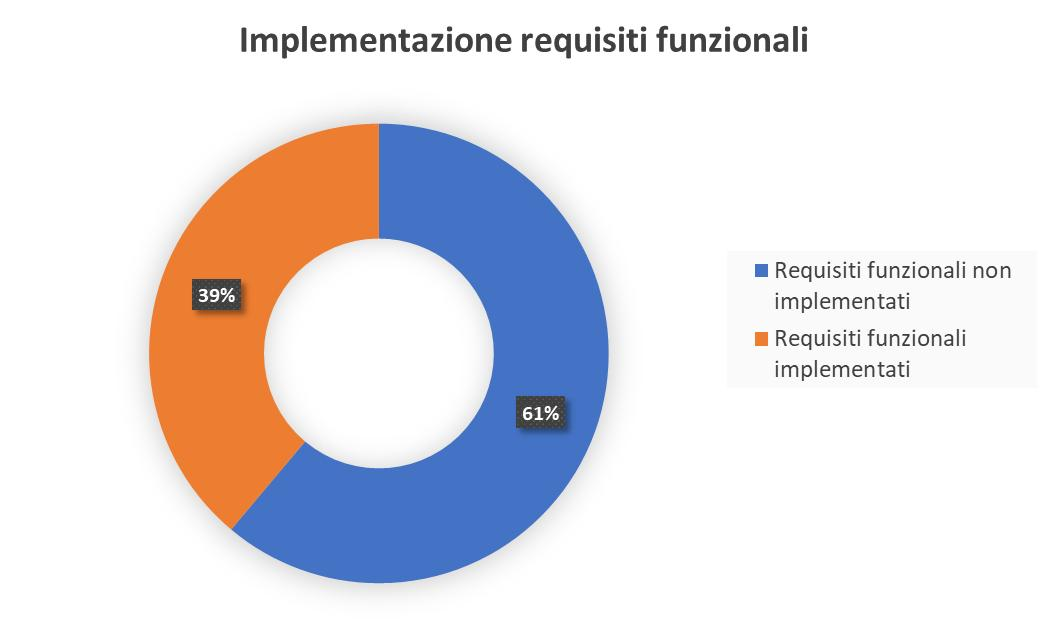
\includegraphics[width=\textwidth,height=\textheight,keepaspectratio]{./img/Grafici/implementazione_requisiti_funzionali.jpg}
            \caption{Grafico implementazione requisiti funzionali}
        \end{figure}
        \begin{figure}[H]
            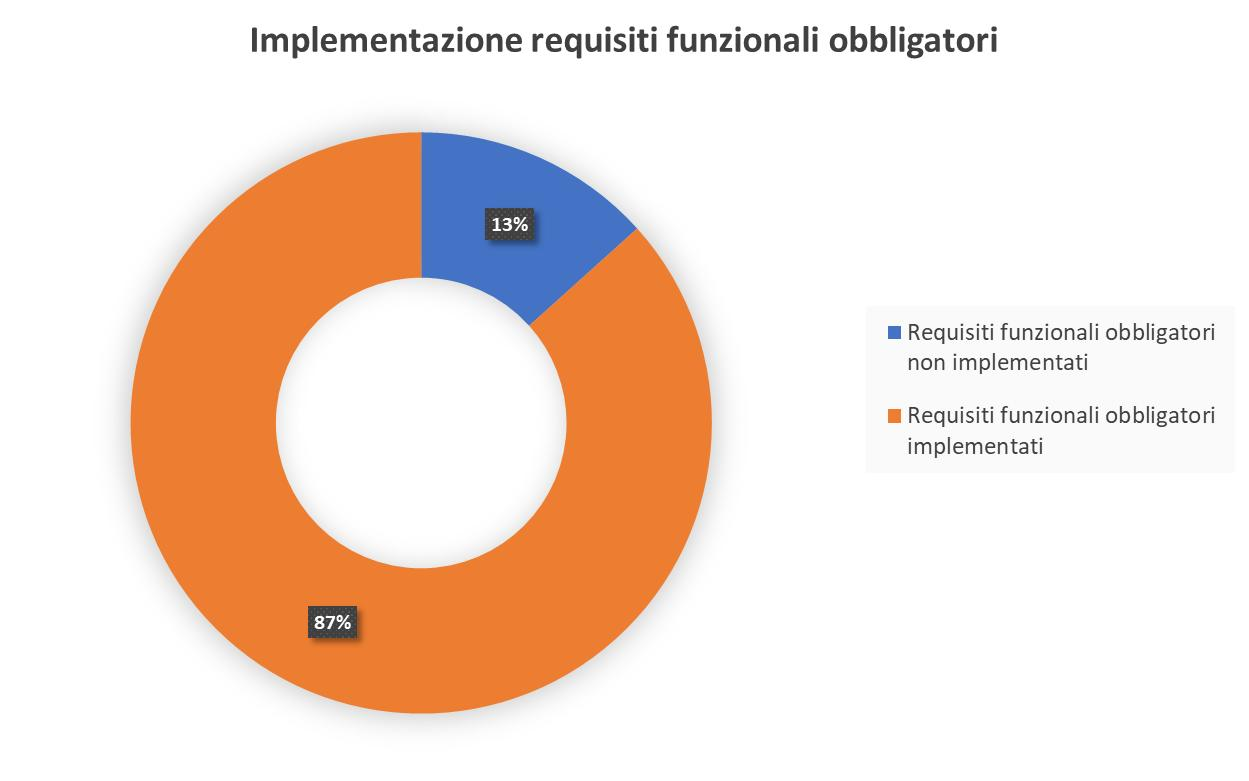
\includegraphics[width=\textwidth,height=\textheight,keepaspectratio]{./img/Grafici/implementazione_requisiti_funzionali_obbligatori.jpg}
            \caption{Grafico implementazione requisiti funzionali obbligatori}
        \end{figure}
    \subsection{Tracciamento requisiti qualitativi}
        \rowcolors{2}{gray!25}{gray!15}
        \begin{longtable} {
            >{\centering}p{64.5mm} 
            >{}p{64.5mm}
            }
        \rowcolor{gray!50}
            \textbf{Requisito} & \textbf{Implementazione} \TBstrut \\
            R1Q1 & Implementato \TBstrut \\ [2mm]
            R1Q2 & Implementato \TBstrut \\ [2mm]
            R1Q10 & Implementato \TBstrut \\ [2mm]
            R1Q3 & Implementato \TBstrut \\ [2mm]
            R1Q4 & Implementato \TBstrut \\ [2mm]
            R1Q5 & Implementato \TBstrut \\ [2mm]
            R2Q6 & Implementato \TBstrut \\ [2mm]
            R1Q7 & Implementato \TBstrut \\ [2mm]
            R1Q8 & Implementato \TBstrut \\ [2mm]
            R1Q9 & Implementato \TBstrut \\ [2mm]
            R1Q11 & Implementato \TBstrut \\ [2mm]
            \rowcolor{white}
            \caption{Tracciamento implementazione requisiti qualitativi}
        \end{longtable}
        \begin{figure}[H]
            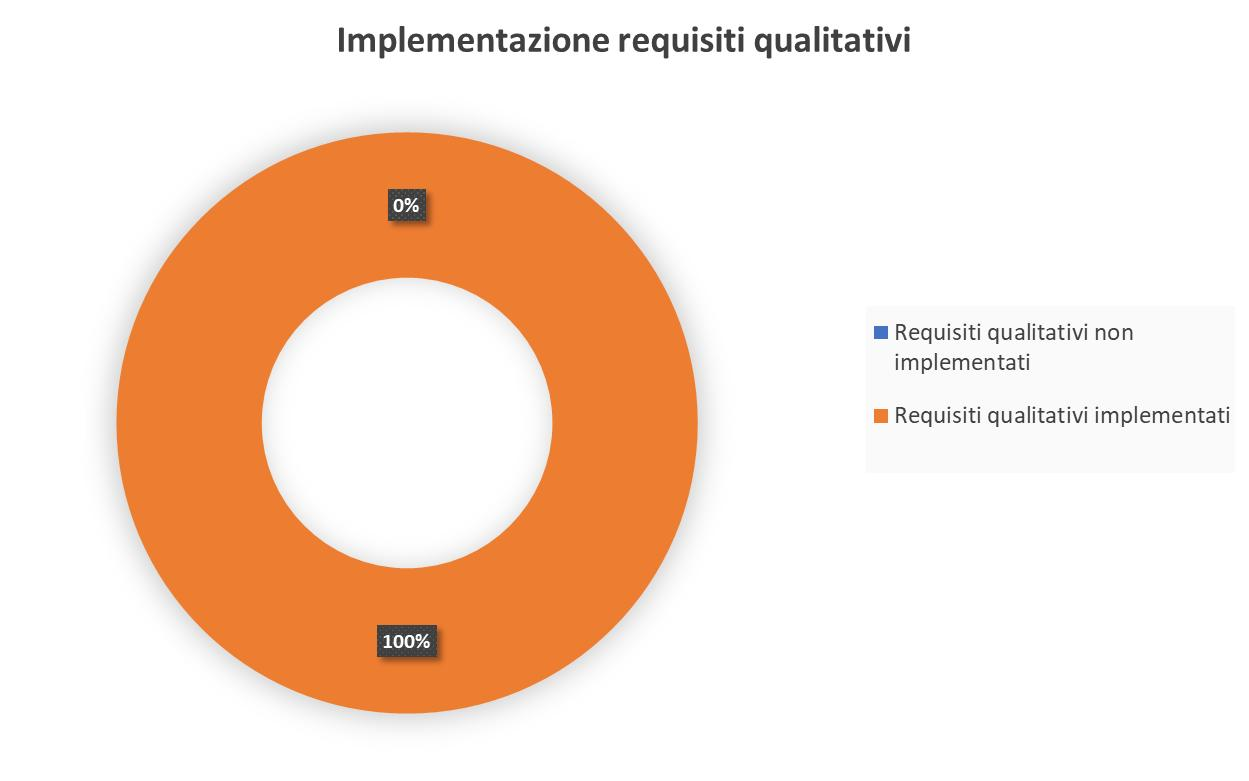
\includegraphics[width=\textwidth,height=\textheight,keepaspectratio]{./img/Grafici/implementazione_requisiti_qualitativi.jpg}
            \caption{Grafico implementazione requisiti qualitativi}
        \end{figure}
        \begin{figure}[H]
            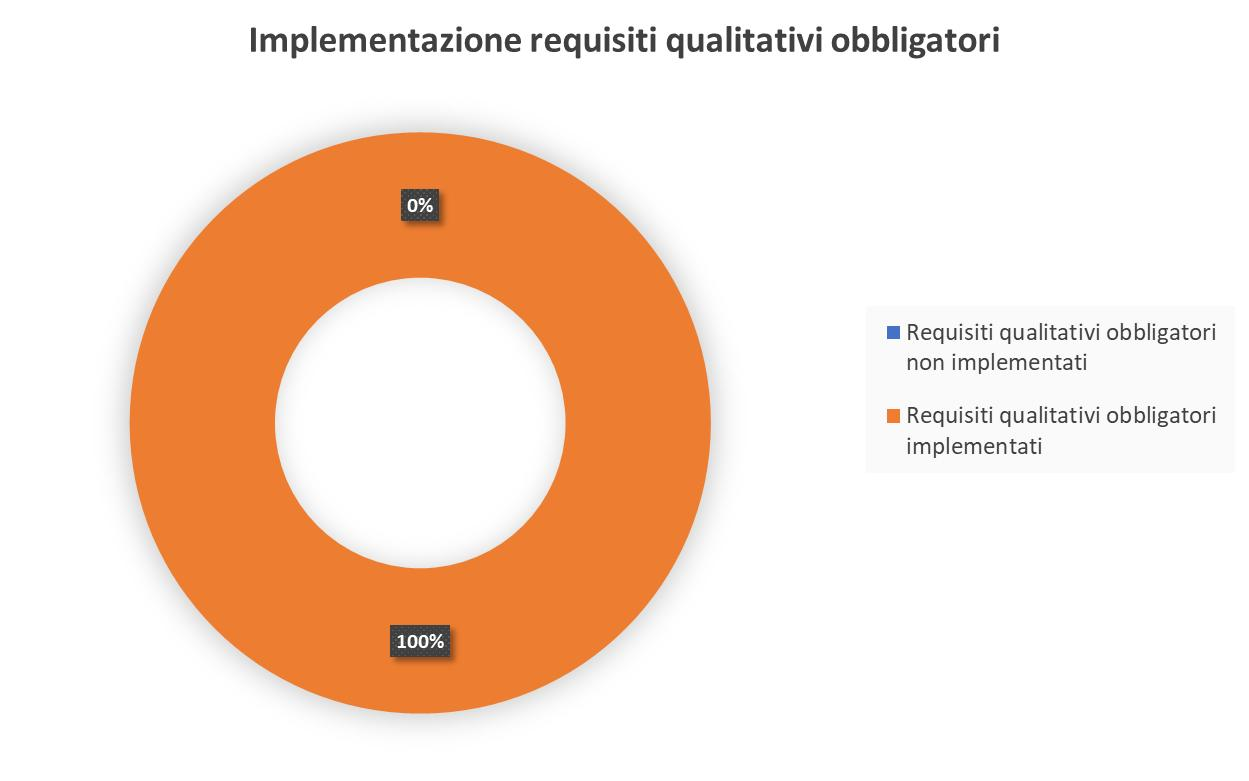
\includegraphics[width=\textwidth,height=\textheight,keepaspectratio]{./img/Grafici/implementazione_requisiti_qualitativi_obbligatori.jpg}
            \caption{Grafico implementazione requisiti qualitativi obbligatori}
        \end{figure}
    \subsection{Tracciamento casi d'uso}
        \rowcolors{2}{gray!25}{gray!15}
        \begin{longtable} {
            >{\centering}p{64.5mm} 
            >{}p{64.5mm}
            }
        \rowcolor{gray!50}
            \textbf{Caso d'uso} & \textbf{Implementazione} \TBstrut \\
            UC1 & Non implementato \TBstrut \\ [2mm]
            UC1.1 & Non implementato \TBstrut \\ [2mm]
            UC1.2 & Non implementato \TBstrut \\ [2mm]
            UC1.3 & Non implementato \TBstrut \\ [2mm]
            UC1.4 & Non implementato \TBstrut \\ [2mm]
            UC1.5 & Non implementato \TBstrut \\ [2mm]
            UC1.6 & Non implementato \TBstrut \\ [2mm]
            UC1.7 & Non implementato \TBstrut \\ [2mm]
            UC1.8 & Non implementato \TBstrut \\ [2mm]
            UC1.9 & Non implementato \TBstrut \\ [2mm]
            UC1.10 & Non implementato \TBstrut \\ [2mm]
            UC1.11 & Non implementato \TBstrut \\ [2mm]
            UC1.12 & Non implementato \TBstrut \\ [2mm]
            UC1.13 & Non implementato \TBstrut \\ [2mm]
            UC1.14 & Non implementato \TBstrut \\ [2mm]
            UC2 & Non implementato \TBstrut \\ [2mm]
            UC2.1 & Non implementato \TBstrut \\ [2mm]
            UC2.2 & Non implementato \TBstrut \\ [2mm]
            UC2.3 & Non implementato \TBstrut \\ [2mm]
            UC3 & Non implementato \TBstrut \\ [2mm]
            UC4 & Implementato \TBstrut \\ [2mm]
            UC4.1 & Implementato\TBstrut \\ [2mm]
            UC4.2 & Implementato \TBstrut \\ [2mm]
            UC4.3 & Implementato \TBstrut \\ [2mm]
            UC4.4 & Implementato \TBstrut \\ [2mm]
            UC4.5 & Implementato \TBstrut \\ [2mm]
            UC4.6 & Implementato \TBstrut \\ [2mm]
            UC4.7 & Implementato \TBstrut \\ [2mm]
            UC4.8 & Implementato \TBstrut \\ [2mm]
            UC4.9 & Implementato \TBstrut \\ [2mm]
            UC4.10 & Implementato \TBstrut \\ [2mm]
            UC4.11 & Implementato \TBstrut \\ [2mm]
            UC4.12 & Non implementato \TBstrut \\ [2mm]
            UC4.13 & Non implementato \TBstrut \\ [2mm]
            UC4.14 & Non implementato \TBstrut \\ [2mm]
            UC4.15 & Non implementato \TBstrut \\ [2mm]
            UC5 & Non implementato \TBstrut \\ [2mm]
            UC5.1 & Non implementato \TBstrut \\ [2mm]
            UC5.2 & Non implementato \TBstrut \\ [2mm]
            UC5.3 & Non implementato \TBstrut \\ [2mm]
            UC6 & Non implementato \TBstrut \\ [2mm]
            UC7 & Implementato \TBstrut \\ [2mm]
            UC8 & Implementato \TBstrut \\ [2mm]
            UC9 & Implementato \TBstrut \\ [2mm]
            UC9.1 & Implementato \TBstrut \\ [2mm]
            UC9.2 & Implementato \TBstrut \\ [2mm]
            UC9.3 & Implementato \TBstrut \\ [2mm]
            UC9.4 & Implementato \TBstrut \\ [2mm]
            UC10 & Non implementato \TBstrut \\ [2mm]
            UC12 & Implementato \TBstrut \\ [2mm]
            UC13 & Non implementato \TBstrut \\ [2mm]
            UC13.2 & Non implementato \TBstrut \\ [2mm]
            UC13.3 & Non implementato \TBstrut \\ [2mm]
            UC13.4 & Non implementato \TBstrut \\ [2mm]
            UC14 & Non implementato \TBstrut \\ [2mm]
            UC15 & Non implementato \TBstrut \\ [2mm]
            UC16 & Non implementato \TBstrut \\ [2mm]
            UC17 & Non implementato \TBstrut \\ [2mm]
            UC18 & Non implementato \TBstrut \\ [2mm]
            UC19 & Implementato \TBstrut \\ [2mm]
            UC20 & Implementato \TBstrut \\ [2mm]
            UC21 & Implementato \TBstrut \\ [2mm]
            \rowcolor{white}
            \caption{Tracciamento implementazione casi d'uso\glo}
        \end{longtable}
        \begin{figure}[H]
            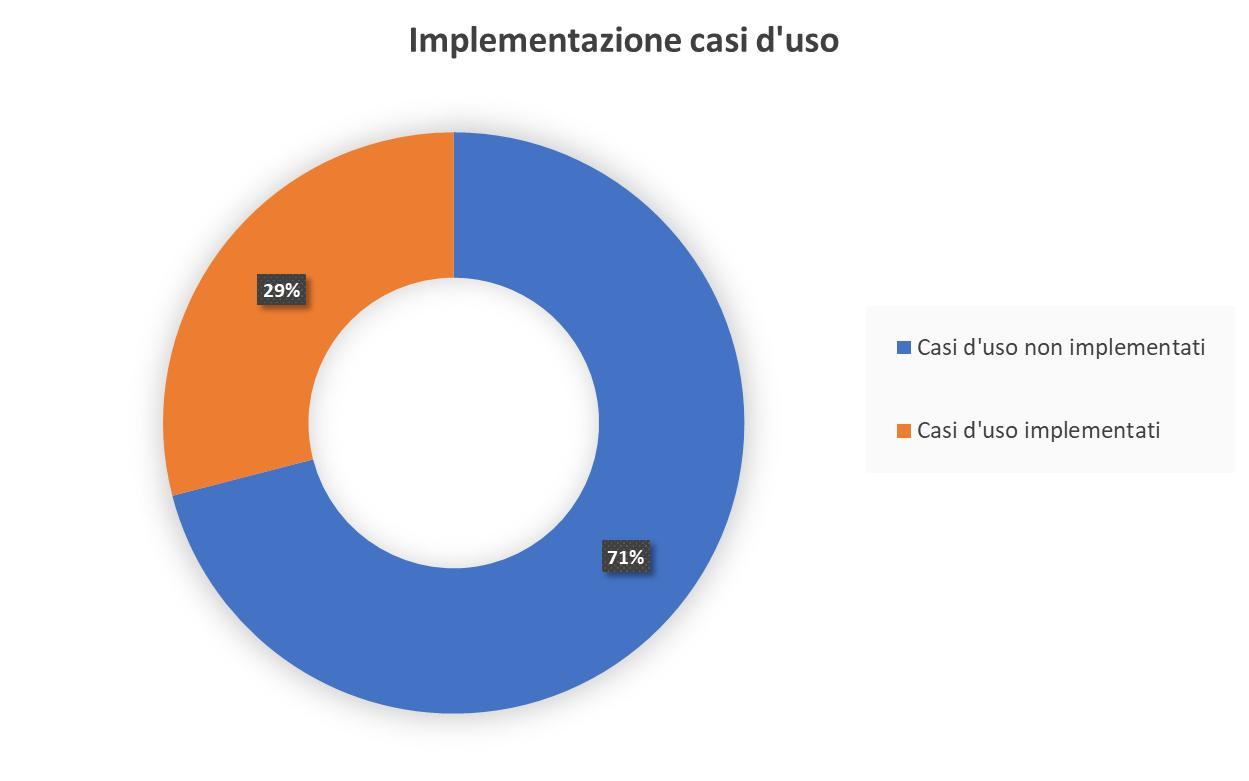
\includegraphics[width=\textwidth,height=\textheight,keepaspectratio]{./img/Grafici/implementazione_casi_d'uso.jpg}
            \caption{Grafico implementazione casi d'uso\glo}
        \end{figure}
	
	%Input del file "decision_table" della cartella locale "res/"
	%% \textbf = grassetto; \Large = font più grande
% \rowcolors{quanti colori alternare}{colore numero riga pari}{colore numero riga dispari}: colori alternati per riga
% \rowcolor{color}: cambia colore di una riga
% p{larghezza colonna}: p è un tipo di colonna di testo verticalmente allineata sopra, ci sarebbe anche m che è centrata a metà ma non è precisa per questo utilizzo TBStrut; la sintassi >{\centering} indica che il contenuto della colonna dovrà essere centrato
% \TBstrut fa parte di alcuni comandi che ho inserito in config.tex che permetto di aggiungere un po' di padding al testo
% \\ [2mm] : questra scrittura indica che lo spazio dopo una break line deve essere di 2mm

%\setcounter{secnumdepth}{0}
%\hfill \break
%\textbf{\Large{Diario delle modifiche}} \\
\section{Riepilogo tracciamenti}
\rowcolors{2}{gray!25}{gray!15}
\begin{longtable} {
		>{\centering}p{17mm} 
		%>{\centering}p{19.5mm}
		%>{\centering}p{24mm} 
		%>{\centering}p{24mm} 
		>{}p{120mm}}
	\rowcolor{gray!50}
	\textbf{Codice} & \multicolumn{1}{c}{\textbf{Decisione}} \\%\textbf{Decisione} \\ %\TBstrut \\
	VI\_1.1 & Scelto \textit{VRAM Software} come nome del gruppo. \TBstrut \\ [2mm]
	VI\_1.1 & Scelto \textit{VRAM Software} come nome del gruppo. \TBstrut \\ [2mm]
	VI\_1.1 & Scelto \textit{VRAM Software} come nome del gruppo. \TBstrut \\ [2mm]
	
\end{longtable} %Tabella delle decisioni (solo per i verbali)
\end{document}